I was given the task to design an LLC Converter as per the following specifications:

\begin{itemize}
    \item Input Voltage to LLC (From PFC) = 400V DC (with 10V ripple)
    \item Output Voltage Range = 42V - 65V DC
    \item Output Power = 1.8kW
\end{itemize}
\noindent
Here's a step-by-step process of how I designed the LLC:

\subsection{Transformer Turn Ratio}
The turn ratio of the transformer is given by the ratio of number of turns on the primary side, and the number of turns on the secondary side, i.e., $n_1 / n_2$, where,\\
$n_1$ is the number of turns at primary side,\\
$n_2$ is the number of turns at secondary side.\\
\\
Let $n = n_1 / n_2 =$ transformer turn ratio, $M_g =$ gain of LLC\\
We know that,
\begin{center}
    $n = M_g * (\frac{V_{in_{nom}}}{V_{out_{nom}}}) * (\frac{1}{2})$
\end{center}
Where,\\
$V_{in_{nom}}$ = Nominal Input Voltage = 400V DC\\
$V_{out_{nom}}$ = Nominal Output Voltage = 52V DC\\
$M_g$ = Gain of LLC = 1 (unity) ; We take it as 1 for this calculation since we want our converter to operate at resonance at nominal output voltage.\\
We multiplied by $1/2$ because we are using a half-bridge configuration.
\\
Therefore,
\begin{center}
    $n = 1 * (\frac{400}{52}) * (\frac{1}{2}) = 3.846$\\
\end{center}

\subsection{LLC Gain}
Now we need to calculate the maximum and minimum gains that we require for our LLC converter. These gain values are calculated W.R.T. the nominal output voltage.\\
$V_{out_{min}} = 42V, V_{out_{max}} = 65V$\\
$V_{in_{nom}} = 400V, V_{in_{min}} = 390V, V_{in_{max}} = 410V$ (PFC Output)\\
Since,
\begin{center}
    $V_{out} = V_{in} * (\frac{1}{2}) * M_g * \frac{1}{n}$
\end{center}
We get,
\begin{center}
    $M_g = 2n * \frac{V_{out}}{V_{in}}$
\end{center}
Hence,
\begin{center}
    $M_{g_{min}} = 2n * \frac{V_{out_{min}}}{V_{in_{max}}} = 2 * 3.846 * \frac{42}{410} = 0.788$\\
    $M_{g_{max}} = 2n * \frac{V_{out_{max}}}{V_{in_{min}}} = 2 * 3.846 * \frac{65}{390} = 1.283$\\
\end{center}
So, we need the gain of the LLC to be between 0.788 and 1.283

\subsection{Equivalent Resistance}
Next step is to calculate the equivalent resistance of the transformer, the rectifier circuit and the load resistance as per the FHA method (First Harmonic Approximation)\\
We require this step as we are replacing the non-linear part of the circuit with an equivalent resistor across the LLC such that the loading of the resistor is same as that of the non-linear part.\\
We know that,
\begin{center}
    $R_{ac} = (\frac{n_1}{n_2})^2 * \frac{8}{\pi^2} * R_L$\\
\end{center}
Also, $R_L = \frac{V_{out_{nom}}^2}{Power} = 1.502\Omega$\\
Hence,
\begin{center}
    $R_{ac} = 3.846^2 * \frac{8}{\pi^2} * 1.502 = 18.03\Omega$\\
\end{center}

\subsection{Choosing value of m}
I will be using a value of m = 6.5 (because we can take any value between 6-10 generally and then we can design our system accordingly).\\
\href{https://www.youtube.com/watch?v=qDT5xw1kgZs&t=391s}{Here is a video that explains the effect of changing m.} (Ctrl / Cmd + Click)\\
Basically, m is the ratio of the magnetizing inductance to the leakage inductance of the transformer.\\
A lower value of m will have much more gain at a particular frequency considering everything else is kept constant, while a larger value of m dampens the frequency - gain curve. (Figure \ref{fig:m_effect})\\
\begin{figure}[H]
    \centering
    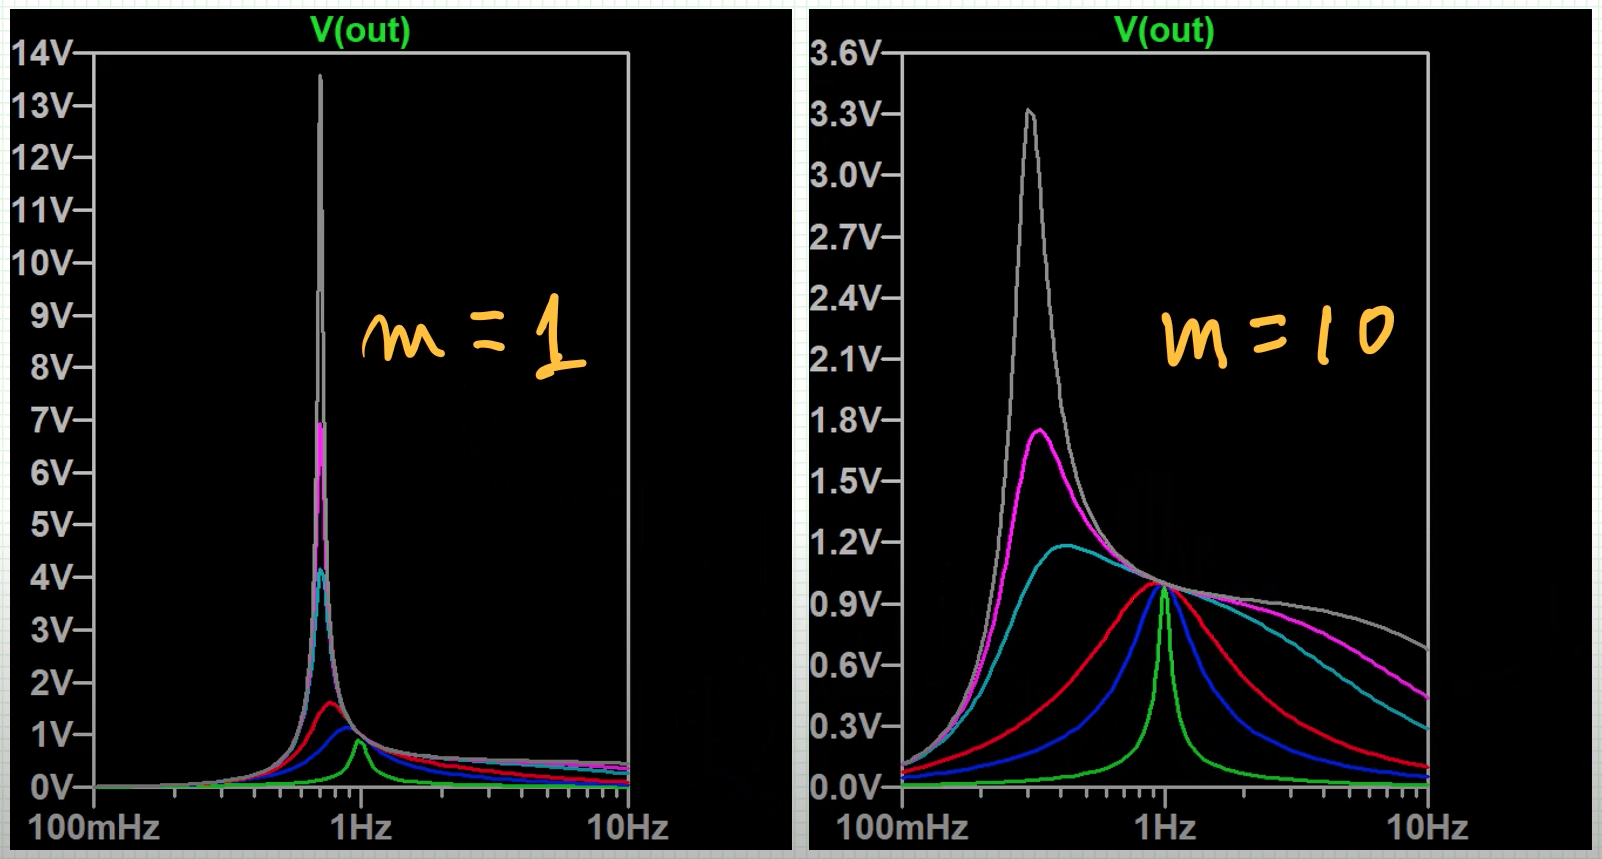
\includegraphics[width=0.8\textwidth]{images/m_effect.png}
    \caption{Effect of m on Frequency-Gain Curve}
    \label{fig:m_effect}
\end{figure}
\noindent
Note: This is a starting point our design. Later on, after other values such as $L_r$, $C_r$ etc. are calculated, we can tune this value further as per our requirements to either minimise losses and hence improving efficiency, or get more gain from the LLC tank.

\subsection{LLC Values}
As per the given values, (assuming $f_r = 127kHz$ because that is the same frequency that we use for 110V system and usually a resonant frequency for LLC is taken between 100-150kHz) the frequency – gain curve according to this setup is as follows (Figure \ref{fig:image4}):
\begin{figure}[H]
    \centering
    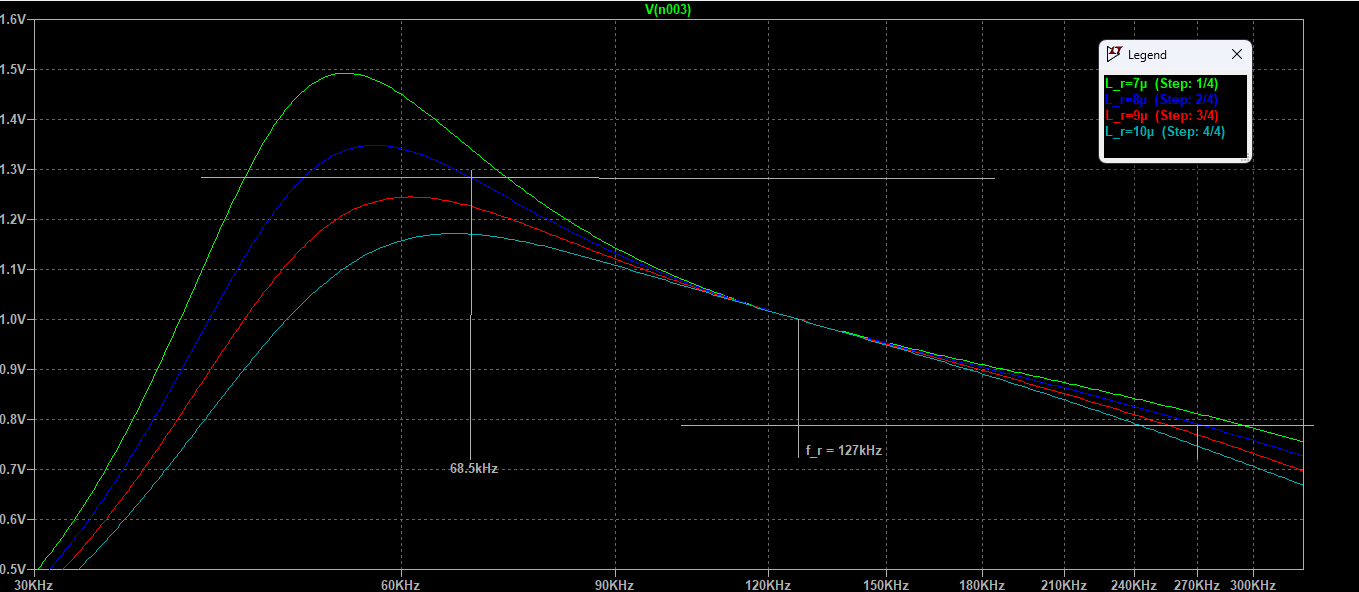
\includegraphics[width=\textwidth]{images/image4.png}
    \caption{Gain-Frequency Plot for 48V-1.8kW LLC Converter}
    \label{fig:image4}
\end{figure}
\begin{itemize}
    \item The upper horziontal line represents the maximum gain of 1.283
    \item The lower horziontal line represents the minimum gain of 0.788
    \item The vertical lines at the intersection of the horizontal lines with the curve represent the maximum and minimum operating frequencies of the converter respectively.
\end{itemize}
As per the graph, $L_r$ values more than $8\mu H$ are of no use as they do not reach the maximum gain that we require.\\
Hence a value of $L_r = 8\mu H$ is chosen. (We can also go for $L_r = 7\mu H$ if we wish to have some room for more gain, but theoritically, $8\mu H$ is the most optimal value with the given conditions and our chosen value of $m = 6.5$)\\
The operating frequency of the converter is from $68.5kHz$ to $270kHz$.
We can calculate the remaining values of the LLC tank from the equations mentioned in Figure \ref{fig:f-gain-circuit}.